\documentclass[11pt]{article}
\usepackage[margin=1in]{geometry}
\usepackage[T1]{fontenc}
\usepackage[utf8]{inputenc}
\usepackage{lmodern}
\usepackage{amsmath}
\usepackage{booktabs}
\usepackage{graphicx}
\usepackage{caption}
\usepackage{float}
\usepackage[hidelinks]{hyperref}
\captionsetup{font=small,labelfont=bf}
\graphicspath{{figures/}}
\newcommand{\GST}{Ge$_2$Sb$_2$Te$_5$}

\title{Melt-quench of \GST{} with 0--10 at.\% carbon:\\ amorphous structure from an Allegro potential}
\author{Part 2 results, \texttt{cgst\_allegro\_sims}}
\date{November 2026}

\begin{document}
\maketitle

\begin{abstract}
Amorphous \GST{} with 0, 1.07, 2.54, 5.14 and 9.96 at.\% C was made by melt-quench molecular dynamics with the Allegro
machine-learned potential run5\_ep301 in 12.4k--13.8k-atom cells, three replicas per composition at 10\,K/ps and one
at 1\,K/ps for 0 and 10\% C. Carbon lowers the density (by 2.2\% in the glass at 10\% C) and the apparent melting
point (1129 to 984\,K), and it segregates: at 10\% C, 91\% of C atoms bond to other C atoms, forming an extended
network. The glass-transition temperature shows no trend resolvable with three replicas. Ge stays mostly
octahedrally coordinated, with a tetrahedral share that grows slightly with C. Quenching at 1\,K/ps partially
crystallizes the glass, so the recrystallization study (Part 3) uses the 10\,K/ps glasses.
\end{abstract}

\section{Method}
The starting structures are $3\times3\times3$ rocksalt supercells of \GST{} with C on cation-vacancy sites; the
10\% C cell has every vacancy filled, so it differs from the others in vacancy count as well as C content. All runs
are NPT at 0\,bar (isotropic Nos\'e--Hoover, $T_\text{damp}=100\,\Delta t$, $P_\text{damp}=1000\,\Delta t$,
$\Delta t=2$\,fs):

\begin{table}[H]
\centering
\begin{tabular}{lll}
\toprule
Stage & Temperature & Duration \\
\midrule
Minimize and equilibrate the crystal & 300\,K & 20\,ps \\
Heat & 300 $\to$ 1500\,K & 120\,ps (10\,K/ps) \\
Melt; MSD gate: every species $\geq 100$\,\AA$^2$ & 1500\,K & 100\,ps \\
Quench & 1500 $\to$ 300\,K & 120\,ps (10\,K/ps) or 1200\,ps (1\,K/ps) \\
Glass: relax, then average & 300\,K & 50 + 50\,ps \\
\bottomrule
\end{tabular}
\end{table}

Coordination uses fixed bond cutoffs (3.2\,\AA{} between Ge/Sb/Te, 2.5\,\AA{} for C--Ge/Sb/Te, 1.9\,\AA{} for C--C);
the C cutoffs were checked on the production 10\% C glass (Section~\ref{sec:cutoffs}). Crystal-like order is
\texttt{xfracGST}, the fraction of Ge/Sb/Te atoms with at least four crystal-like Steinhardt-$q_4$ bonds (criterion
3.6\,\AA, 0.5, 4). All 17 runs passed the melt gate with the same 100\,ps hold.

\section{Thermodynamic properties}

\begin{table}[H]
\centering
\caption{Properties against C content, 10\,K/ps, mean $\pm$ sample standard deviation over three replicas.}
\begin{tabular}{lccccc}
\toprule
C (at.\%) & $\rho_\text{liquid}$, 1500\,K & $\rho_\text{glass}$, 300\,K & $T_{m,\text{app}}$ (K) & $T_g$ (K) &
\texttt{xfracGST}, 300\,K \\
 & (g/cm$^3$) & (g/cm$^3$) & & & \\
\midrule
0    & $5.524 \pm 0.001$ & $6.289 \pm 0.004$ & $1129 \pm 2$  & $807 \pm 26$ & $0.155 \pm 0.006$ \\
1.07 & $5.524 \pm 0.001$ & $6.277 \pm 0.003$ & $1128 \pm 13$ & $780 \pm 22$ & $0.144 \pm 0.008$ \\
2.54 & $5.514 \pm 0.001$ & $6.260 \pm 0.001$ & $1117 \pm 5$  & $833 \pm 53$ & $0.139 \pm 0.002$ \\
5.14 & $5.493 \pm 0.000$ & $6.221 \pm 0.002$ & $1077 \pm 26$ & $757 \pm 45$ & $0.133 \pm 0.009$ \\
9.96 & $5.444 \pm 0.002$ & $6.148 \pm 0.002$ & $984 \pm 35$   & $815 \pm 57$ & $0.143 \pm 0.010$ \\
\bottomrule
\end{tabular}
\label{tab:props}
\end{table}

\begin{figure}[htbp]
\centering
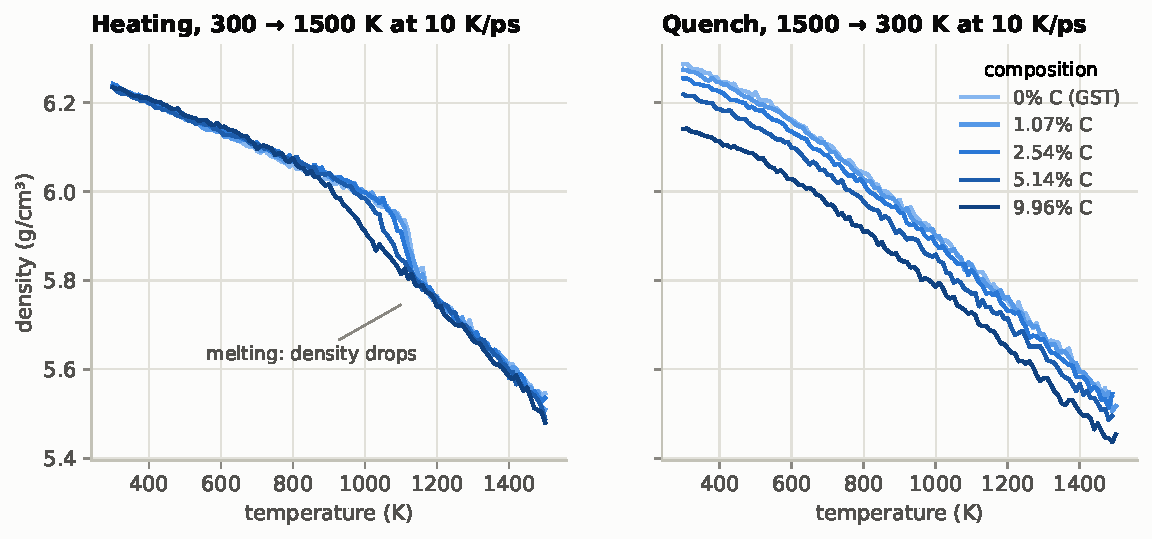
\includegraphics[width=\textwidth]{density_vs_T.pdf}
\caption{Density on the 10\,K/ps heating ramp (left; the drop near 1100\,K is melting of the superheated crystal)
and on the quench (right), mean of three replicas per composition.}
\label{fig:rhoT}
\end{figure}

\begin{figure}[htbp]
\centering
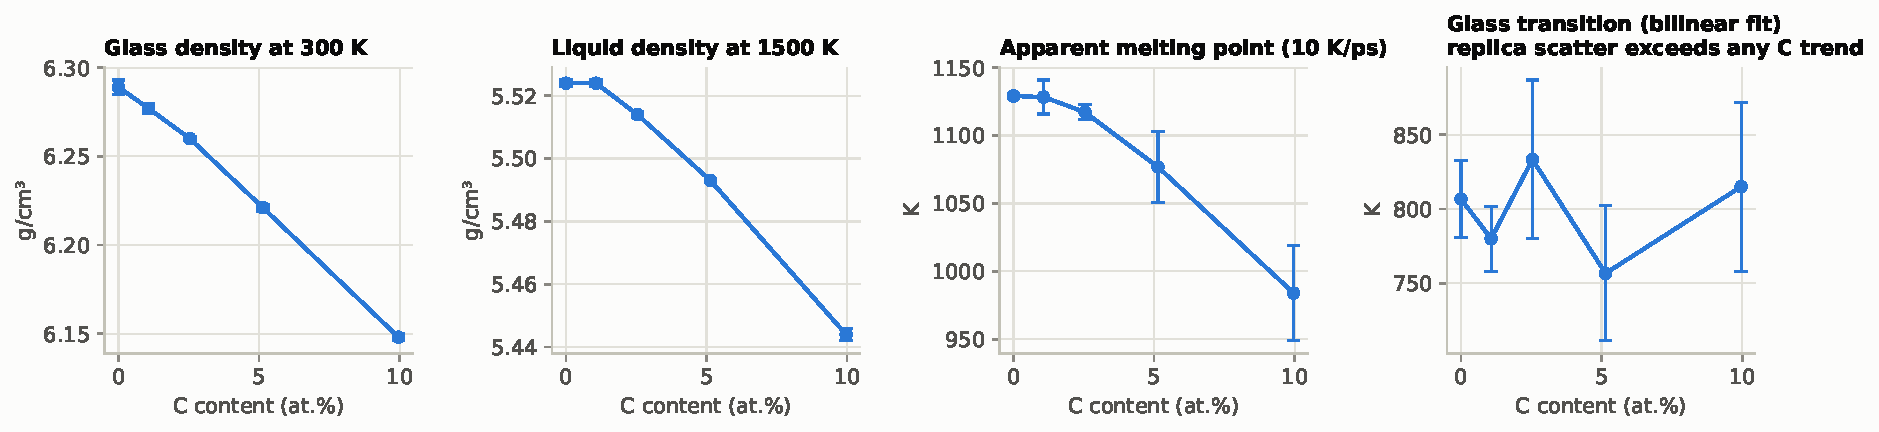
\includegraphics[width=\textwidth]{properties_vs_C.pdf}
\caption{Glass and liquid density, apparent melting point and glass transition against C content (Table~\ref{tab:props}).}
\label{fig:props}
\end{figure}

Density falls with C steadily and well outside the replica spread: by 1.4\% in the liquid and 2.2\% in the glass from 0
to 10\% C (Fig.~\ref{fig:props}). The apparent melting point, the temperature of fastest enthalpy rise on the 10\,K/ps
heating ramp, falls above 2.5\% C, from 1129 to 984\,K; it is a superheating limit and thus an upper bound on the
model's melting point, and its spread grows with C. The glass transition from a bilinear fit of $V(T)$ on the quench
scatters by 20--60\,K between replicas, more than any difference between compositions, so the effect of C on $T_g$ is
not resolved at this rate and replica count. Crystal-like order in the glass falls slightly with C, to 0.133 at 5\% C;
the 10\% C cell, the vacancy-free endpoint, reads 0.143.

\section{Structure of the glass}

\begin{figure}[htbp]
\centering
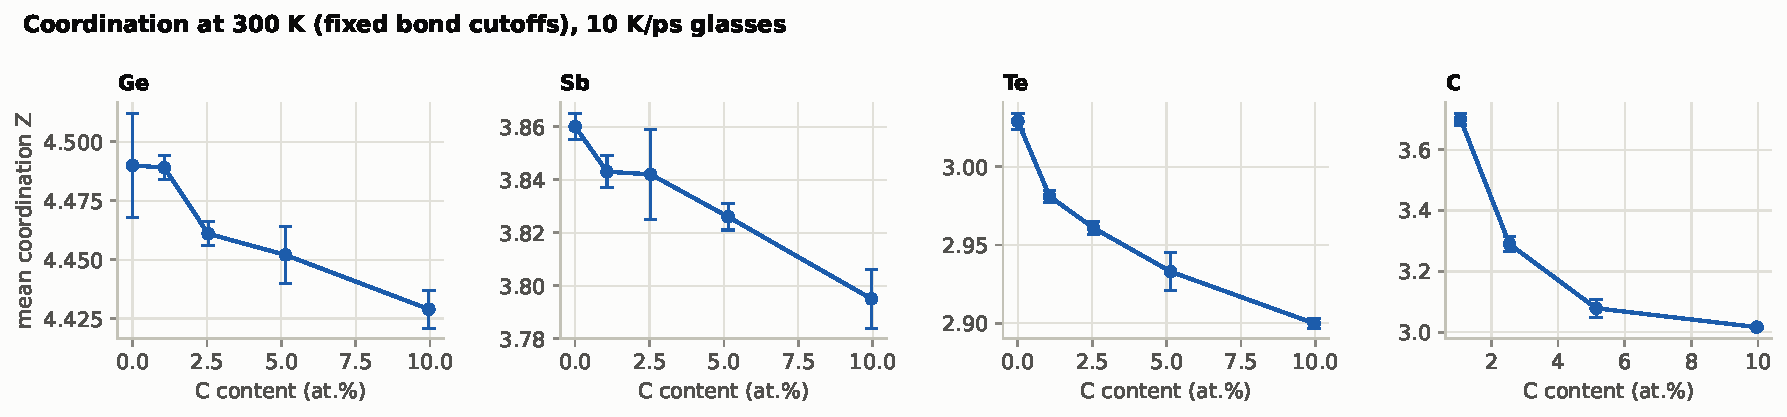
\includegraphics[width=\textwidth]{coordination_vs_C.pdf}
\caption{Mean coordination of each species at 300\,K against C content.}
\label{fig:coord}
\end{figure}

\begin{figure}[htbp]
\centering
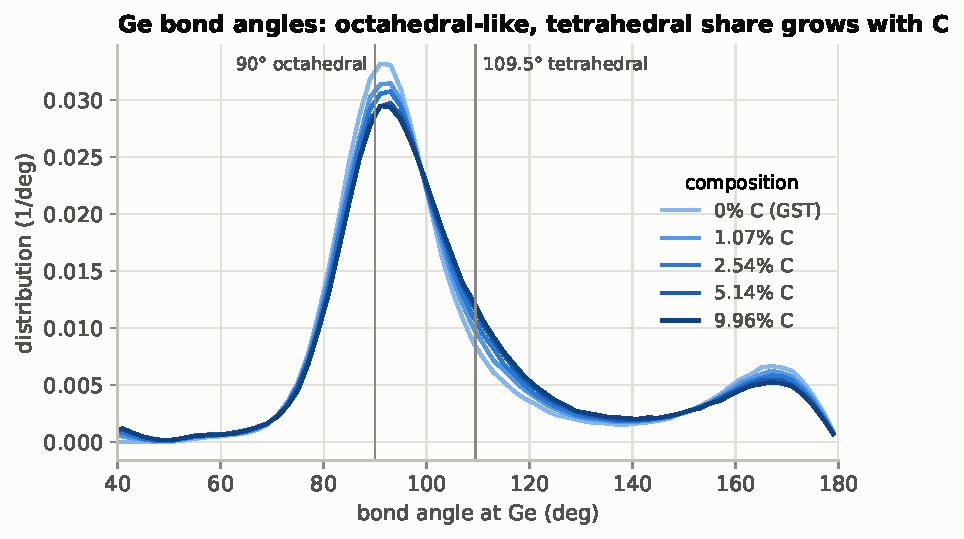
\includegraphics[width=0.49\textwidth]{ge_angles.pdf}\hfill
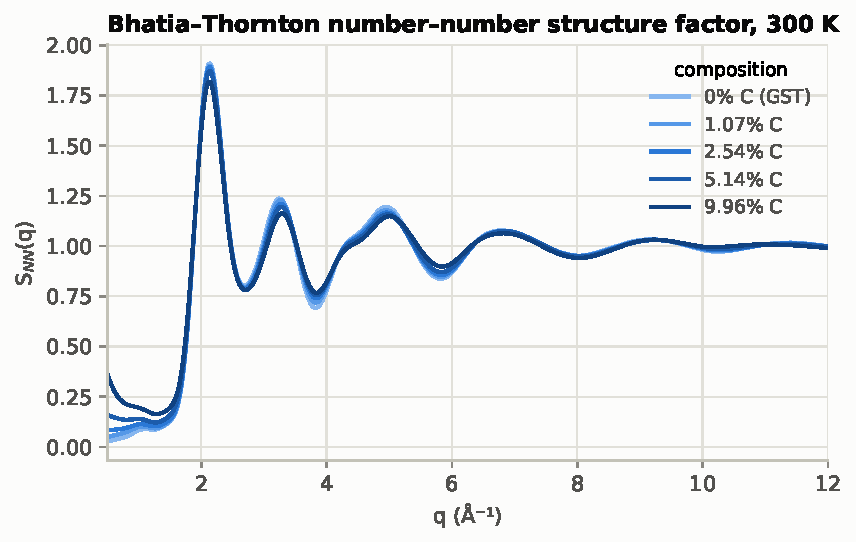
\includegraphics[width=0.49\textwidth]{sq_nn.pdf}
\caption{Left: bond-angle distribution at Ge. Right: Bhatia--Thornton number--number structure factor $S_{NN}(q)$.}
\label{fig:angles}
\end{figure}

Coordination drops slightly with C (Fig.~\ref{fig:coord}): Ge from 4.49 to 4.43, Sb from 3.86 to 3.80, Te from 3.03 to
2.90. C is 3.70-coordinated at 1\% C and 3.02 at 10\%. The Ge bond-angle distribution peaks at 91--93$^\circ$
(octahedral-like) for every composition, while the share between 100 and 120$^\circ$ (tetrahedral-like) rises from
0.19 to 0.25 with C (Fig.~\ref{fig:angles}). $S_{NN}(q)$ barely changes beyond 2\,\AA$^{-1}$; it rises at low $q$
with C, most for 10\% C, consistent with the larger-scale density fluctuations of a segregated C network (not analysed
further).

\section{Carbon clustering}

\begin{figure}[htbp]
\centering
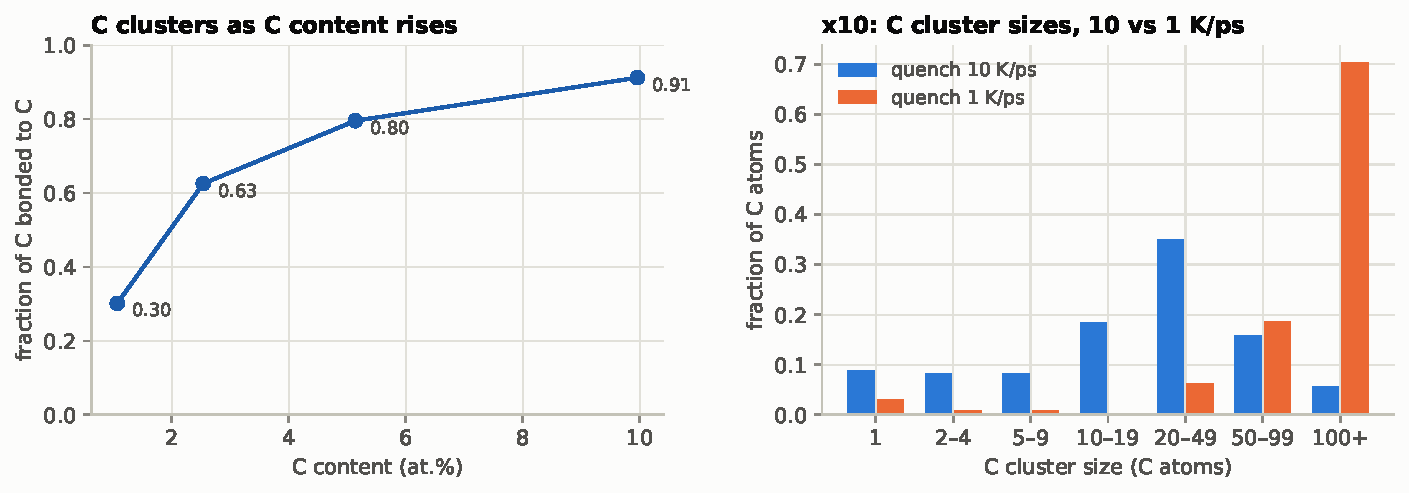
\includegraphics[width=\textwidth]{carbon_clustering.pdf}
\caption{Left: fraction of C atoms bonded to at least one other C. Right: C cluster sizes in the 10\% C glass after
10 and 1\,K/ps quenches.}
\label{fig:cclust}
\end{figure}

\begin{figure}[htbp]
\centering
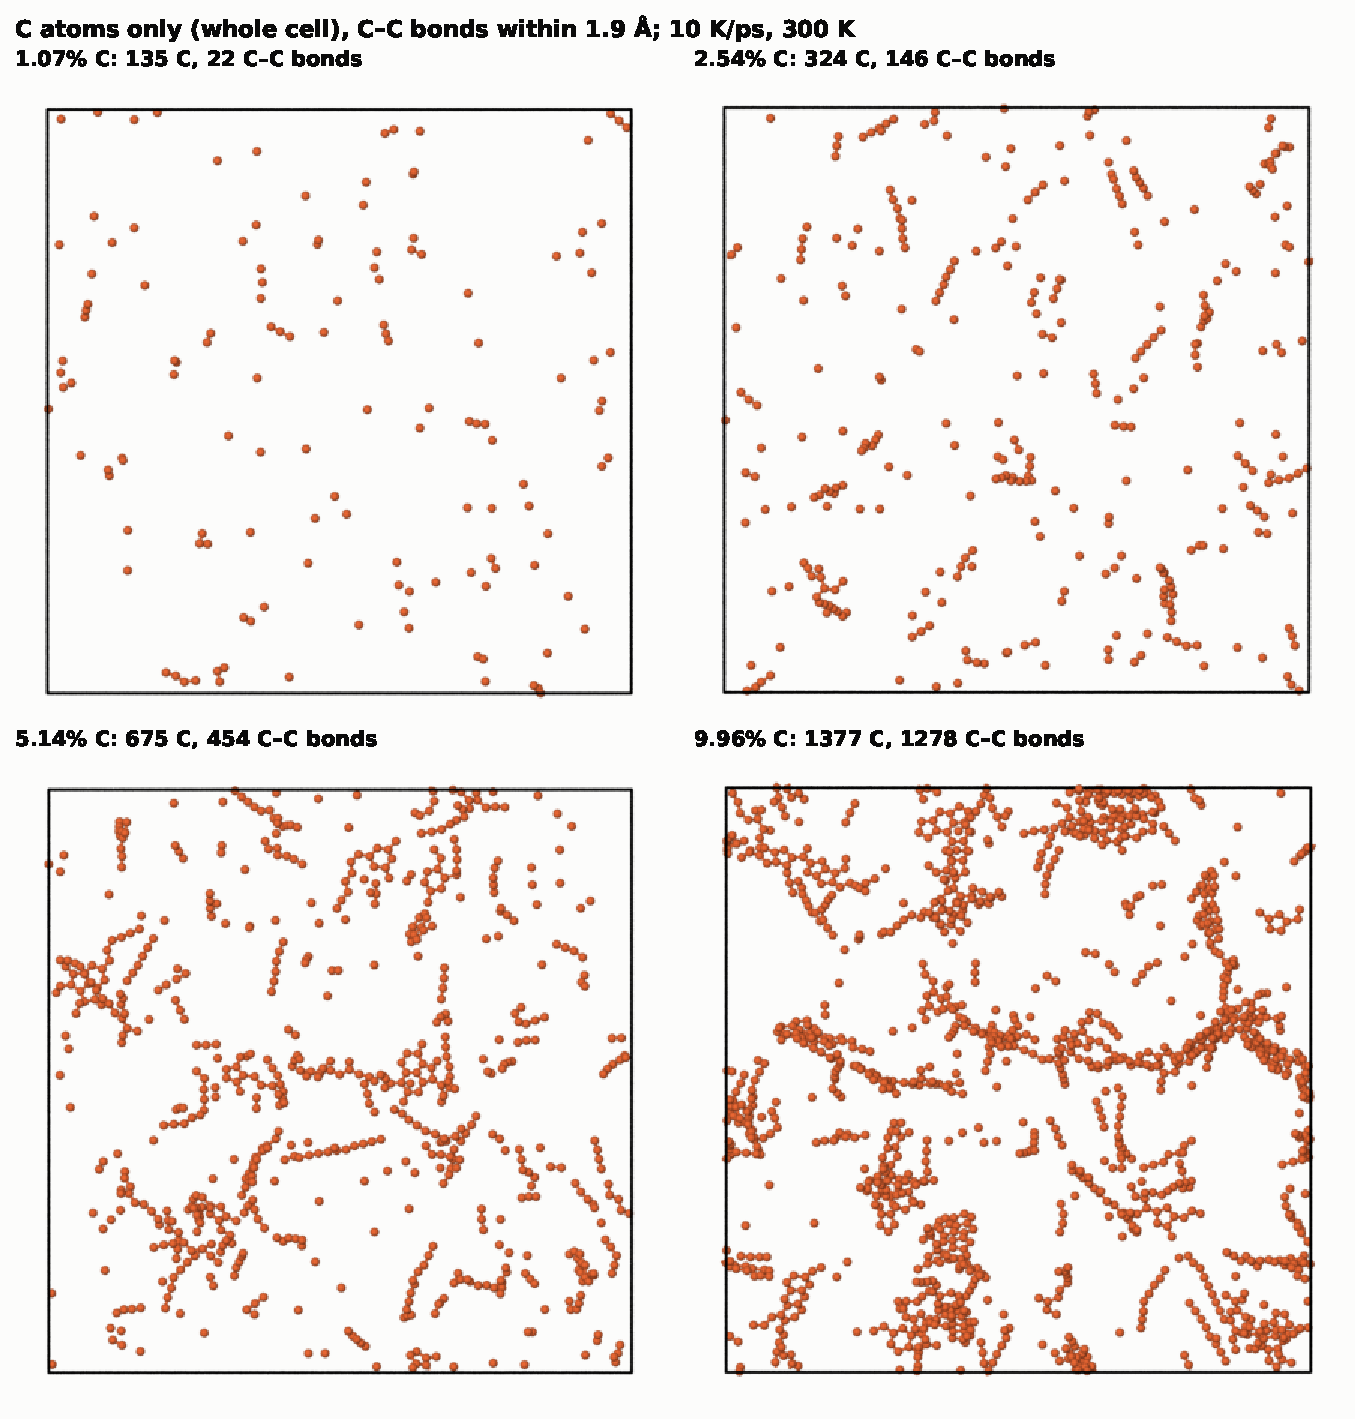
\includegraphics[width=0.78\textwidth]{render_c_network_all_grid.pdf}
\caption{C atoms only (whole cell seen along $z$) in the 10\,K/ps glasses at 300\,K, 1.07 to 9.96\% C; C--C bonds
within 1.9\,\AA. The projection makes some depth overlaps look like contacts.}
\label{fig:cnetall}
\end{figure}

\begin{figure}[htbp]
\centering
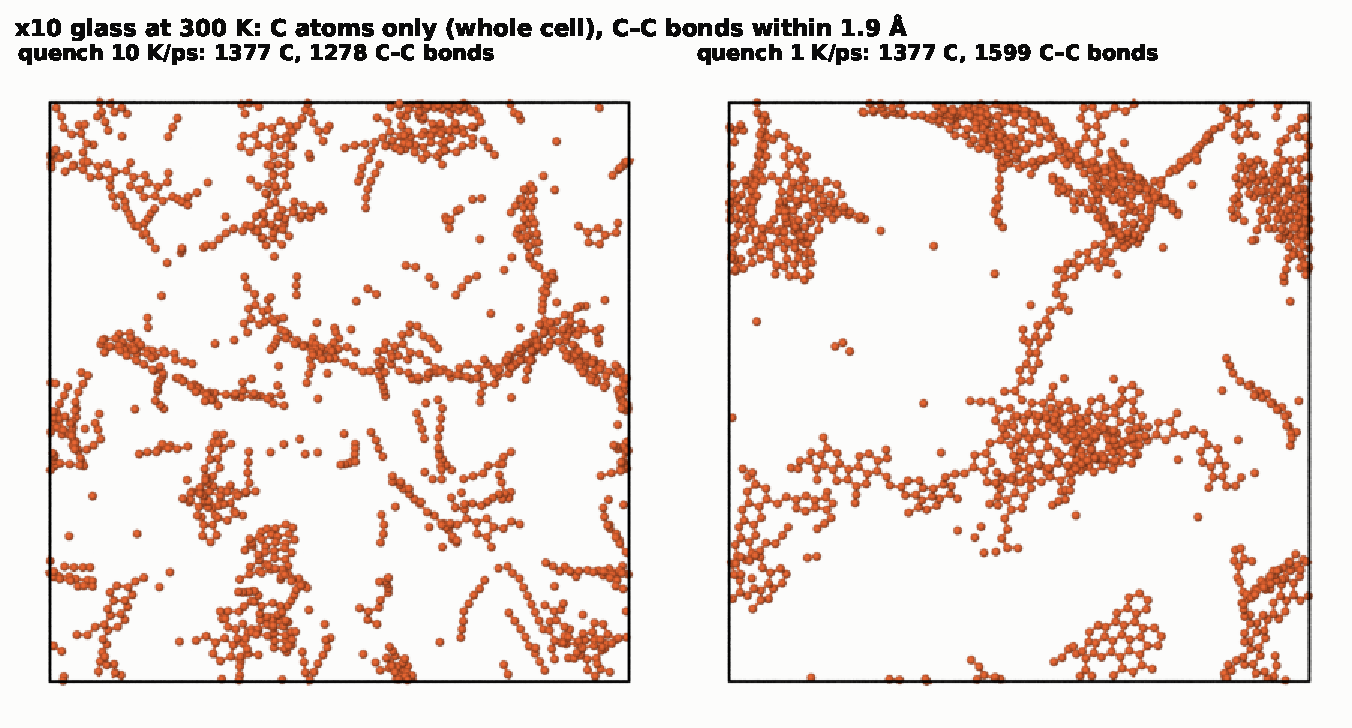
\includegraphics[width=0.72\textwidth]{render_c_network.pdf}
\caption{The 10\% C glass at 300\,K after 10 and 1\,K/ps quenches, C atoms only, whole cell seen along $z$.}
\label{fig:cnet}
\end{figure}

\begin{figure}[htbp]
\centering
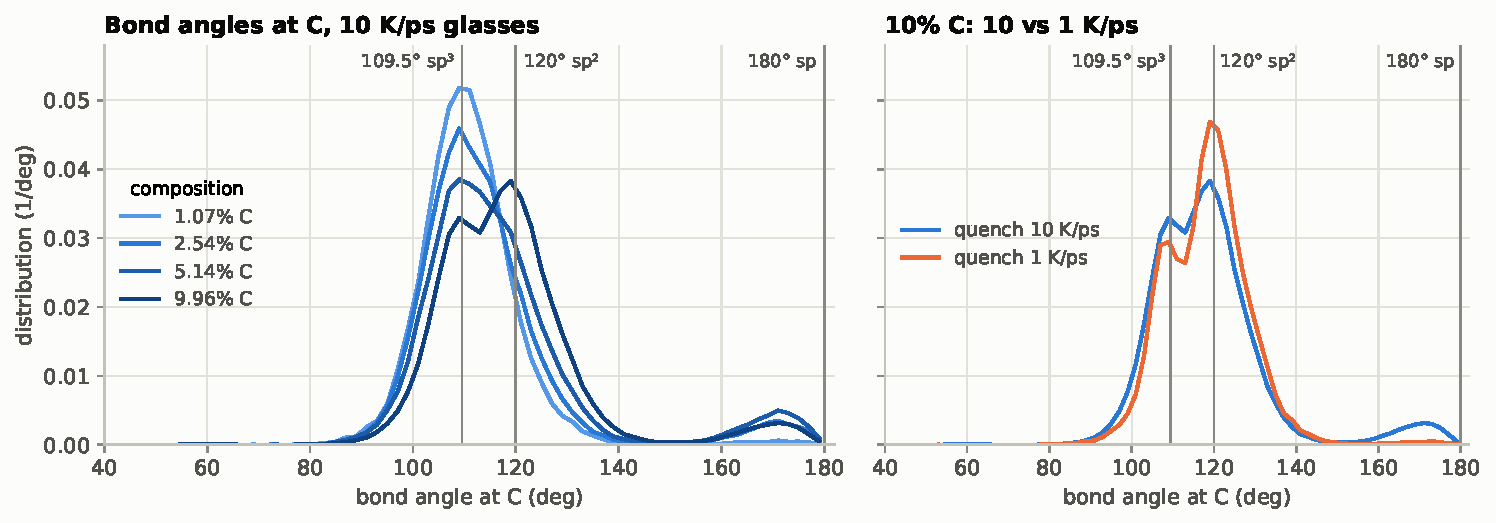
\includegraphics[width=\textwidth]{c_angles.pdf}
\caption{Bond-angle distribution at C. Left: 10\,K/ps glasses, 1.07 to 9.96\% C. Right: 10\% C after 10 and
1\,K/ps quenches. Reference lines at the tetrahedral (sp$^3$), planar (sp$^2$) and linear (sp) angles.}
\label{fig:cang}
\end{figure}

The fraction of C atoms bonded to another C rises from 0.30 at 1\% C through 0.63 and 0.80 to 0.91 at 10\% C
(Fig.~\ref{fig:cclust}). At 10\% C, 75\% of C sits in clusters of ten or more atoms, up to 129, so carbon forms an
extended network inside the glass rather than dispersed dopant atoms (Figs.~\ref{fig:cnetall} and
\ref{fig:cnet}): isolated C atoms and dimers at 1\% C give way to short chains by 2.5\% and to branched, connected
clusters at 5--10\%, with 0.34, 0.90, 1.35 and 1.84 C--C bonds per C atom. The commonest C
environments change from Ge/Sb-rich (Ge$_3$Sb 19\%, Ge$_2$C 13\%, Ge$_2$Sb$_2$ 12\% at 1\% C) to C-rich (C$_3$ 22\%,
GeC$_2$ 21\%, C$_2$ 15\% at 10\% C). C binds Ge before Sb before Te: in the 10\% C glass there are 0.40 C neighbours
per Ge atom, 0.12 per Sb and 0.03 per Te.

C bonding also changes character (Fig.~\ref{fig:cang}). At 1\% C the C-centred bond angles peak at 109$^\circ$,
tetrahedral (sp$^3$-like), with 59\% of angles between 100 and 115$^\circ$. At 10\% C the main peak moves to
119$^\circ$, planar (sp$^2$-like), with 48\% between 115 and 130$^\circ$, as C increasingly bonds to other C; this
matches the fall of C's coordination from 3.70 to 3.02. A 1\,K/ps quench pushes further toward planar bonding (56\%
between 115 and 130$^\circ$), and a small near-linear population near 170$^\circ$ appears from 2.5\% C at 10\,K/ps.

\section{Quench rate}

\begin{figure}[htbp]
\centering
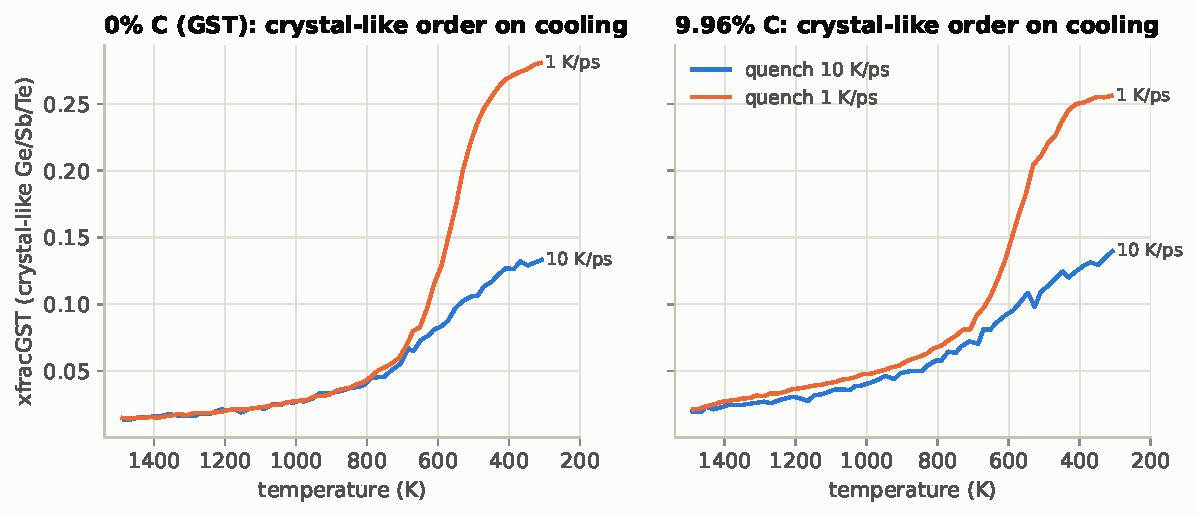
\includegraphics[width=\textwidth]{quench_order.pdf}
\caption{Crystal-like order of Ge/Sb/Te on cooling, 10 against 1\,K/ps, for 0 and 10\% C.}
\label{fig:rate}
\end{figure}

\begin{figure}[htbp]
\centering
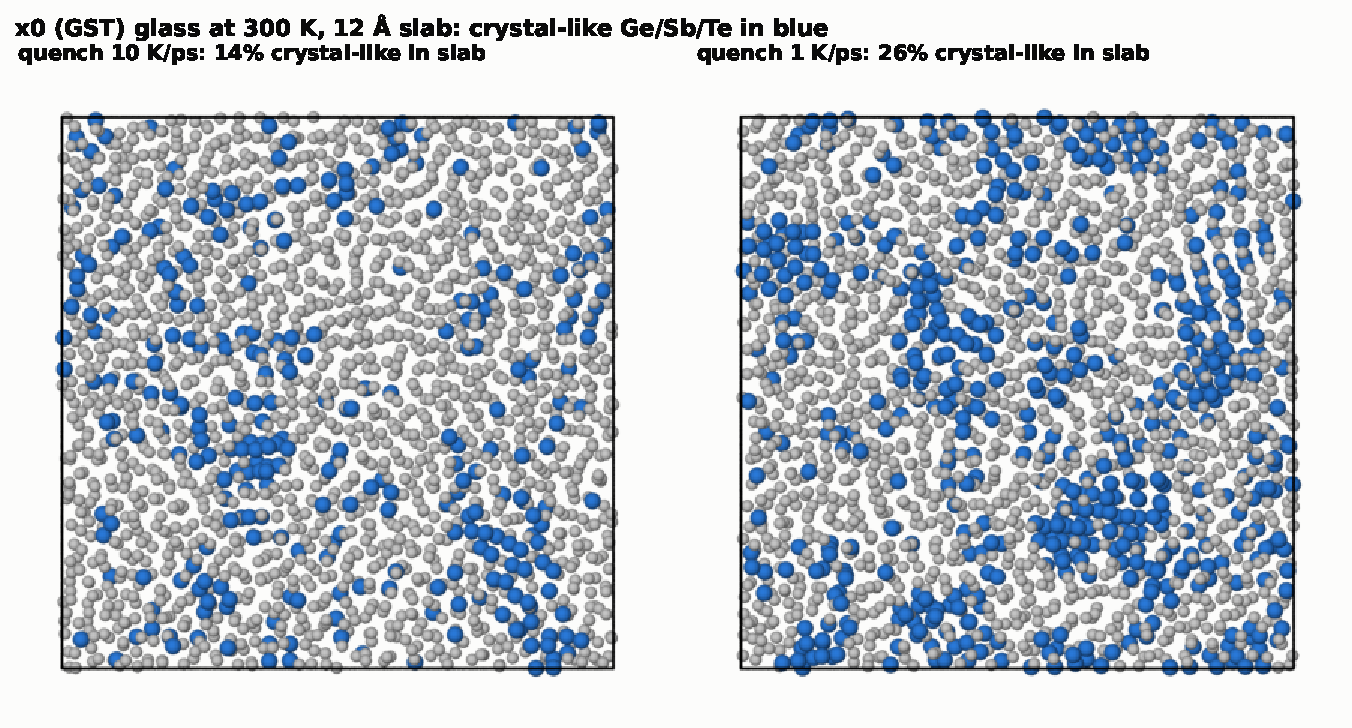
\includegraphics[width=0.9\textwidth]{render_crystal_like.pdf}
\caption{The 0\% C glass at 300\,K, 12\,\AA{} slab: crystal-like Ge/Sb/Te atoms (in-run bond count $\geq 4$) in blue.}
\label{fig:render}
\end{figure}

After a 1\,K/ps quench, \texttt{xfracGST} at 300\,K is 0.28 (0\% C) and 0.26 (10\% C), against 0.13--0.16 after
10\,K/ps, and it rises during the quench between 600 and 400\,K (Fig.~\ref{fig:rate}): the 1\,K/ps glasses are partly
crystallized, not merely better relaxed (Fig.~\ref{fig:render}). Slower quenching also coarsens the C network (95\% of
C in clusters of ten or more, up to 286 atoms). Glass density barely depends on rate (0\% C: 6.283 against
6.289\,g/cm$^3$). The recrystallization study therefore starts from the 10\,K/ps glasses.

\section{Bond-cutoff check}
\label{sec:cutoffs}

\begin{figure}[htbp]
\centering
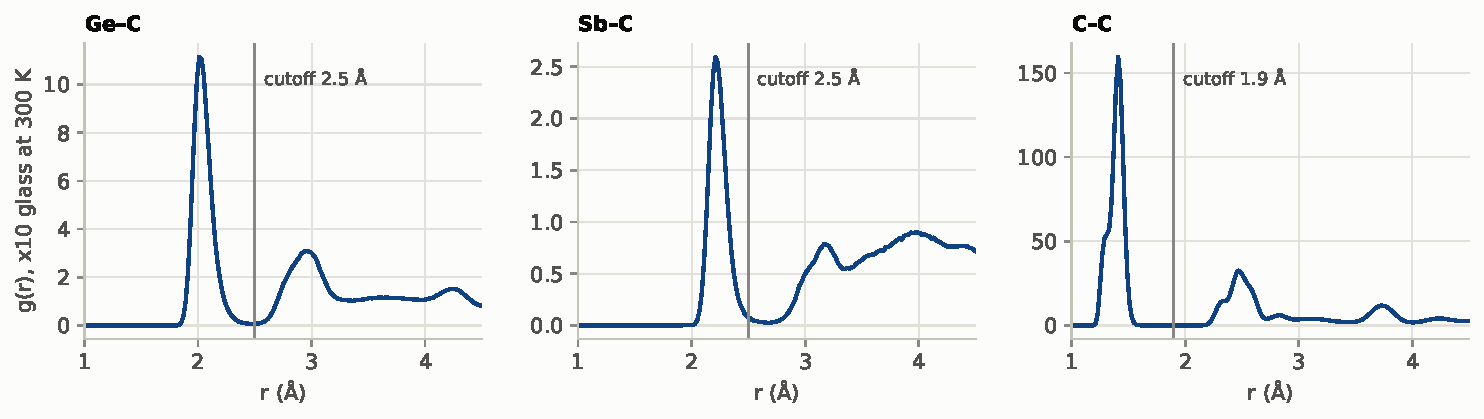
\includegraphics[width=\textwidth]{c_cutoffs.pdf}
\caption{Partial $g(r)$ for C pairs in the 10\% C glass with the fixed bond cutoffs.}
\label{fig:cut}
\end{figure}

The C cutoffs were set on a small test glass and checked on the production 10\% C glasses (Fig.~\ref{fig:cut}):
$g_\text{CC}(1.9\,\text{\AA}) = 0$ in all four. At 2.5\,\AA, $g$ is 0.05--0.09 for Ge--C and Sb--C, on the tails of
peaks at 2.0 and 2.2\,\AA; moving the cutoff by $\pm0.1$\,\AA{} changes the C coordination of Ge by at most 2\% and of
Sb by 4--6\%. The cutoffs were kept.

\section{Limitations}
\begin{itemize}
\item \textbf{Dense glass.} The model's glass (6.29\,g/cm$^3$) is denser than its own crystal (6.24), unlike
experiment, where the glass is about 6--7\% less dense. This is inherited from the DFT training reference, so
conclusions that depend on the glass--crystal density difference belong to that reference.
\item \textbf{Rates.} Both quench rates are many orders of magnitude faster than experiment; $T_{m,\text{app}}$ is a
superheating limit and $T_g$ depends on rate.
\item \textbf{Crystal-like order is not crystallinity.} Even the 10\,K/ps glasses hold crystal-like patches of up to a
few hundred atoms, a baseline the recrystallization analysis accounts for.
\end{itemize}

\end{document}
